
\documentclass[a4paper,12pt]{article}
\usepackage[margin=1in]{geometry}
\renewcommand{\tabcolsep}{1 mm}
\usepackage[T2A]{fontenc}			% кодировка
\usepackage[utf8]{inputenc}			% кодировка исходного текста
\usepackage[english,russian]{babel}	% локализация и переносы
\usepackage{graphicx}                % Математика
\usepackage{amsmath,amsfonts,amssymb,amsthm,mathtools} 
\usepackage{mathtext}
\usepackage[T2A]{fontenc}
\usepackage[utf8]{inputenc}

\usepackage{wasysym}

%Заговолок
\author{Бичина Марина 
группа Б04-005 1 курса ФЭФМ}
\title{Отчет по лабораторной работе №2.2.1


Исследование взаимной диффузии газов}
\date{22.03.2021}


\begin{document} % начало документа

\maketitle
\newpage

\section{Аннотация}

\paragraph{Цель работы:} 
\begin{enumerate}
\itemsep0em
\item регистрация зависимости концентрации гелия в воздухе от времени с помощью датчиков теплопроводности при разных начальных давлениях смеси газов
\item определение коэффициента диффузии по результатам измерений
\end{enumerate}
\paragraph{Оборудование:}
\begin{enumerate}
\itemsep0em
\item измерительная установка
\item форвакуумный насос 
\item баллон с газом (He)
\item манометр
\item источник питания
\item магазин сопротивлений 
\item гальванометр
\item секундомер
\end{enumerate}
\section{Теоретическая часть}

\paragraph{} \textit{Диффузией} называют самопроизвольное взаимное проникновение веществ друг в друга, происходящее вследствие хаотичного теплового движения молекул. При перемешивании молекул разного сорта говорят о \textit{взаимной (концентрационной)} диффузии.

Диффузия в системе, состоящей из двух компонентов $a$ и $b$, подчиняется закону Фика: плотности потока компонентов $j_{a,b}$(количество частиц, пересекающих единичную площадку в единицу времени) пропорциональны градиентам их концентраций $\nabla n_{a, b}$, что в одномерном случае можно записать как:
\begin{equation}
j_a = -D_{ab}\frac{\partial n_a}{\partial x}, 
\;\;\; j_b = -D_{ba}\frac{\partial n_b}{\partial x}
\end{equation} 
где $D_{ab} = D_{ba} = D$ - коэффициент взаимной диффузии компонентов

В данной работе исследуется взаимная диффузия гелия и воздуха. Давление $P$ и температура $T$ в условиях опыта предполагаются неизменными: $P = (n_{He}+n_{B}k_\text{Б},\; T = const$, где $n_{He}, n_{B}$ -- концентрации диффундирующих газов. Поэтому для любых изменений концентраций справедливо $\Delta n_{B} = \Delta n_{He}$. Следовательно, достаточно ограничиться описанием диффузии одного из компонентов (остановимся на гелии)

Приведём теоретическую оценку для коэффициента диффузии. В работе концентрация гелия, как правило, мала $(n_{He}\ll n_{в})$. Кроме того, атомы гелия
существенно легче молекул, составляющих воздух $(\mu_{He}\ll\mu_{N_2},\mu_{O_2})$, значит и их средняя тепловая скорость велика по сравнению с остальными частицами. Поэтому перемешивание газов в работе можно приближенно описывать как диффузию примеси лёгких частиц гелия на практически стационарном фоне воздуха. Коэффициент диффузии в таком приближении равен:
\begin{equation}
D = \frac{1}{3}\lambda\langle v \rangle,
\end{equation}
где $\langle v \rangle = \sqrt{\dfrac{8RT}{\pi\mu}}$ -- средняя тепловая скорость частиц примеси, $\lambda = \dfrac{1}{n_0\sigma}$ -- их длина свободного пробега, $n_0$ -- концентрация рассеивающего фона, $\sigma$ -- сечение столкновения частиц примеси с частицами фона.

В общем случае необходимо учитывать диффузию каждого из
компонентов. Более подробное рассмотрение показывает, что для бинарной смеси формула (2) сохраняется, если:
\begin{enumerate}
\itemsep0em
\item Под $\lambda$ понимать величину $\lambda = \dfrac{1}{n_{\Sigma}\sigma}$, где $n_{\Sigma}=n_{He}+n_{B} = \dfrac{P}{k_{\text{Б}}T}$ -- полная концентрация частиц
\item Под $\langle v \rangle$ понимать среднюю относительную скорость частиц разных сортов.

\end{enumerate}

Таким образом, теория предсказывает, что коэффициент диффузии бинарной смеси обратно пропорционален давлению в системе, и не зависит от пропорций компонентов, что и предлагается проверить в работе экспериментально ($D\propto\frac{1}{P}$)

Для исследования взаимной диффузии используется установка, изображенная на рисунке 1. Два сосуда с примерно одинаковыми объемами $V_1 \approx V_2 \equiv V$ соединены трубкой длины l и сечения S. Сосуды заполнены смесью двух газов при одинаковом давлении, но с различной концентрацией компонентов. Вследствие взаимной диффузии концентрации каждого из компонентов в обоих сосудах с течением времени выравниваются. 

Рассмотрим этот процесс. Решение задачи упрощается, если сделать несколько допущений:
\begin{enumerate}
\itemsep0em
\item Пренебрежем объемом соединительной трубки, поскольку он мал по сравнению с объемами сосудов
\item Концентрацию газов в каждом из сосудов будем считать постоянной по всему объему сосуда
\item Предположим, что процесс выравнивания концентраций происходит в основном благодаря диффузии в трубке
\end{enumerate}
Тогда диффузионный потом в любом сечении трубки одинаков,поэтому $J = -DS(\partial n/ \partial x)$ не меняется вдоль трубки, следовательно:
\begin{equation}
J = -DS\frac{n_1 - n_2}{l}
\end{equation}
Обозначим через $\Delta n_1 \text{и} \Delta n_2$ изменения в объемах V за время $\Delta t$. Тогда $V_1\Delta n_1$ равно изменению количества компонента в объеме $V_1$, a $V_2\Delta n_2$ -- изменению этого компонента в $V_2$. Из закона сохранения вещества $V_1\Delta n_1 = -V_2\Delta n_2$. Тогда получим:
\begin{equation}
V\frac{dn_1}{dt} = -DS\frac{n_1 - n_2}{l}, \;\;\;\;\ V\frac{dn_2}{dt} = DS\frac{n_1 - n_2}{l}
\end{equation}
Вычтя уравнения друг из друга, найдем:
\begin{equation}
\frac{n_1}{dt} - \frac{dn_2}{dt} = -\frac{n_1 - n_2}{l}DS(\frac{2}{V})
\end{equation}
Интегрируя, получим:
\begin{equation}
n_1 - n_2 = (n_1 - n_2)_0 e^{(-t/\tau)}
\end{equation}
где $(n_1 - n_2)_0$ -- разность концентраций в начальный момент времени, 
\begin{equation}
\tau = \dfrac{V}{2}\dfrac{l}{SD}
\end{equation}
 -- постоянная времени процесса, определяемая геометрией установки и величиной коэффициента диффузии D.

Для проверки применимости квазистационарного течения убедимся, что время $\tau$ много больше характерного времени диффузии одной частицы вдоль трубки длиной $l$: $t_{\text{диф}} \sim \frac{l^2}{D} \ll \tau$.

 Для измерения концентраций применяются датчики теплопроводности $D_1$ и $D_2$ (см. рис. 1) и используется зависимость теплопроводности газовой смеси от её состава. Тонкая проволока радиуса $r_{\text{пр}}$, протянутая вдоль оси цилиндра радиуса $R_{\text{ц}}$, нагревается током. Тепло от проволоки к стенке цилиндра передаётся главным образом вследствие теплопроводности газа, находящегося внутри цилиндра. Количество тепла переданного стенке цилиндра в единицу времени, определяется по формуле 
\begin{equation}
Q = \varkappa \frac{2\pi L}{ln (R_{\text{ц}}/r_{\text{пр}})}(T_1-T_2)
\end{equation}
где $\varkappa$ - теплопроводность, $L$ - длина нити, $T_1, T_2$ - температуры проволочки и стенки. При $Q = const$ температура проволоки и её сопротивление определяются теплопроводностью газа и, следовательно, его составом. Для измерения разности концентраций газов используется  
мостовая схема, представленная на рисунке 2 (см. описание установки).
	 
	 При разности концентраций, равной $15\%$, поправка к линейному закону не превышает $0,5\%$, что для наших целей достаточно.
	 
 В процессе диффузии разность концентраций убывает по экспоненциальному закону.
 \begin{equation}
N = N_0e^{-t/\tau}
\end{equation}
 По тому же закону изменяются во времени показания гальванометра:
\begin{equation}
U = U_0e^{-t/\tau}
\end{equation}
Измеряя экспериментально зависимость $U(t)$, можно получить характерное время процесса $\tau$, откуда определить коэффициент диффузии D.

\subsection{Описание установки:}
\begin{figure}[h]
\begin{center}
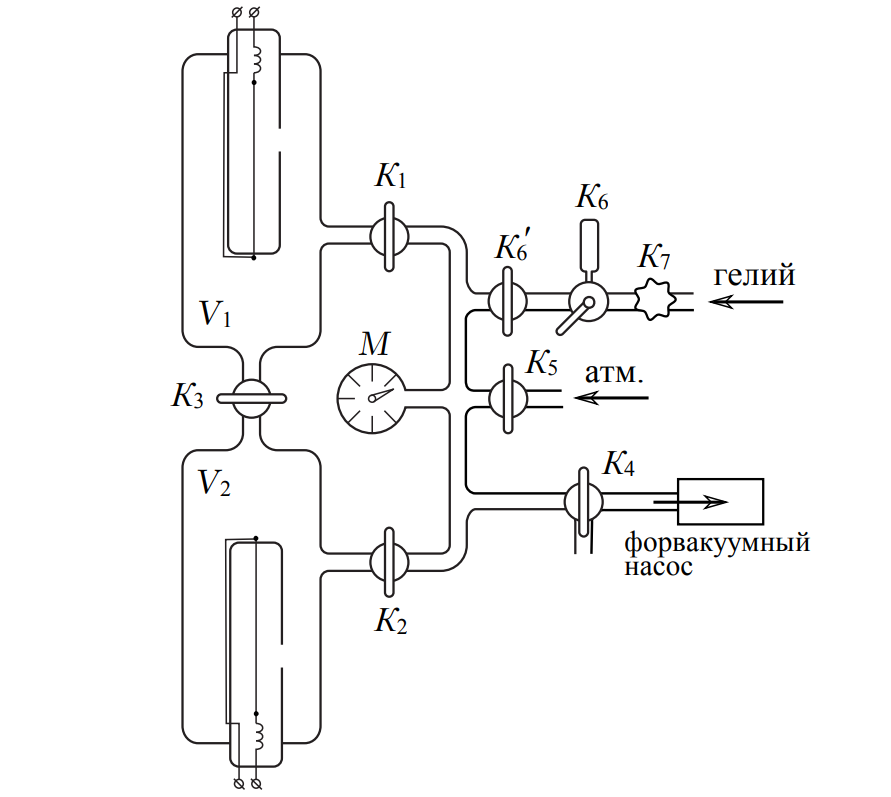
\includegraphics[width=0.5\linewidth]{ustanovka_graph.png}
\label{ris:ustanovka_1} 
\caption{Установка для исследования взаимной диффузии газов}
\end{center}
\end{figure}
\paragraph{}
Установка состоит из двух сосудов $V_1 \approx V_2 \equiv V$, соединенных краном $K_3$, форвакуумного насоса, манометра М и системы напуска гелия, включающей в себя краны $K_6, \; K'_6,\; K_7$. Дополнительный кран $K'_6$ служит для вакуумной изоляции установки от системы подачи гелия. Для подачи воздуха в установку служит кран $K_5$. Сосуды $V_1 \; \text{и} \; V_2$ и порознь и вместе можно соединять как с системой напуска гелия, так и с форвакуумным насосом. Для этого служат краны $K_1,\; K_2,\; K_4,\; K_5$. Манометр М регистрирует давление газа, до которого заполняют тот или другой сосуды. Краны $K_4,\; K_5 \; \text{и} \; K'_6$ обладают повышенной вакуумплотностью и хорошо изолируют установку от протечек.

В силу того, что в сосуд требуется подавать малое давление гелия, кран $K_6$ снабжен дозатором. Подробный разрез крана $K_6$ приведен на рисунке 3.

На рисунке 2 приведена схема электричского соединения $D_1 \; \text{и} \; D_2$ -- сопротивления проволок датчиков парциального давления, которые состовляют одно плечо моста. Второе плечо моста состовляют сопротивления $r_1, \; R_1, \; r_2, \; R_2, \; r_1 \ll R_1, \; r_2 \ll R_2, \; R_1 \; \text{и} \; R_2$ спаренные, их подвижные контакты находятся на общей оси. Оба они используются для грубой регулировки моста. Точная балансировка моста выполняется потенциометром $R$. Последовательо с гальванометром Г, стоящим в диагонали моста, поставлен магазин сопротивления $M_R$. Когда мост балансируют, магазин сопротивлений выводят на ноль. 


\begin{figure}[h]
\begin{center}
\begin{minipage}[h]{0.4\linewidth}
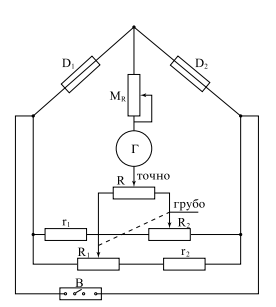
\includegraphics[width=0.8\linewidth]{bridge.png}
\label{bridge}
\caption{Мостовая схема с датчиками теплопроводности для измерения разности концентраций газов} 
\end{minipage}
\hfill
\begin{minipage}[h]{0.5\linewidth}
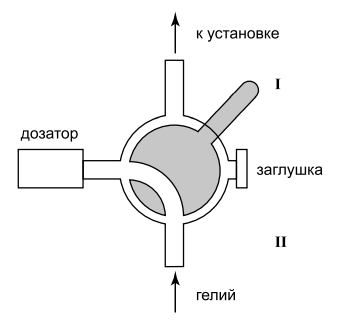
\includegraphics[width=1\linewidth]{K_6.png}
\caption{Кран $K_6$}
\end{minipage}
\end{center}
\end{figure}

\subsection{Контрольные вопросы:}
\begin{enumerate}
\itemsep0em
\item Показать, что в условиях опыта концентрацию газов можно считать постоянной по всему объему сосуда $V_1$ (и $V_2$)\\
Концентрацию газа в сосуде $V_1$ можно считать равной концентрации в сосуде $V_2$, поскольку по условию мы напускаем в них одинаковое давление. В условиях эксперимента газы идеальные $\Longrightarrow$ мы можем воспользоваться уравнением Менделеева-Клапейрона $PV = \frac{N}{N_{a}}RT$; $P = \frac{\frac{N}{V}RT}{N_{a}}$; $P = \frac{nRT}{N_{a}}$
\item Через какое время после открытия крана $K_3$ диффузионный поток в трубке можно считать одинаковым во всем сечении трубки? \\
Через время, равное $t = 3\tau$, когда разница в концентрациях будет достаточно мала
\item Каким будут результаты опыта, если воздух и гелий поменять местами (например, исходное давление гелия $P = 40$ торр, а воздуха $P = 4$ торр? \\
Коэффициент взаимной диффузии уменьшится, поскольку скорость движения частиц воздуха в несколько раз меньше, чем гелия 

\item Почему следует ожидать, что график зависимости D от 1/P должен иметь вид прямой линии? \\
D зависит от длины свободного пробега $\lambda$, $\lambda$ обратно зависит от концентрации частиц ($\lambda = \frac{1}{\sigma*n}$), а из уравнения Менделеева-Клапейрона давление прямо пропорционально концентрации $P = \frac{nRT}{N_{a}}$
\end{enumerate}
\section{Ход работы:}
\begin{enumerate}
\itemsep0em
\item Ознакомимся со схемой установки. Перепишем параметры установки: 
$$V_1 = V_2 = V = 775 \pm 10 \; \text{см}^{3}, \; \frac{L}{S} = 5,3 \pm 0.1 \; 
\text{см}^{-1}$$ 
проверим, что краны $K_4,\; K_5 \; K'_6$ закрыты перед началом откачки. 
\item Включим питание электрической схемы установки. Откроем краны $K_1$, $K_2$, $K_3$.
Поскольку манометр измеряет разность давления внутри резервуаров с атмосферным в $\frac{\text{кгс}}{\text{cм}^2}$ необходимо записать показание манометра при полностью откачанном сосуде $P_0 = 99,5 \;\dfrac{\text{кгс}}{\text{cм}^2}$ (оно равно атмосферному) и в дальнейшем постоянно вычитать из него показания прибора, тем самым будет найдено давление внутри установки.
\item Очистим установку от всех газов, которые в ней есть. Для этого откроем кран $K_4$. Включим форвакуумный насос  и соединим его с установкой, повернув ручку крана $K_5$ длинным концом рукоятки влево (на установку). Откачаем установку до давления $\approx 0.1 \; \text{торр} $, что достигается непрерывной работой насоса в течение 3–5 минут. Для прекращения откачки ручку крана $K_5$ поставим длинным концом вверх, выключим насос
\item  Напустим в установку воздух до рабочего давления (вначале $P \approx 40 \; \text{торр}$), открыв кран $K_5$, чтобы сбалансировать мост на рабочем давлении. Сбалансируем мост.
\item Заполним установку рабочей смесью согласно порядку предложенному в указании к работе: в сосуде $V_2$ должен быть воздух, а в сосуде $V_1$ — смесь воздуха с гелием.
\item Проведём измерения. Для этого откроем кран $K_3$, заснимем на видео процесс падения напряжения на гальванометре на $40 - 50\%$ Будем продолжать аналогичные измерения при различных значениях $P_\text{раб}$ в интервале $40 - 200$ торр. Результаты измерений сведены в таблицы ниже:
\paragraph{Данные при $P_{\Sigma} = 40$ торр:}

\begin{center}
\begin{tabular}{|l||l|l|l|l|l|l|l|l|l|l|l|l|l|l|l|l|l|l|l|l|l|l|l|l}
\hline
$t,\; \text{c}$ & 5 & 10 & 15 & 20 & 25 & 30 & 35 & 40 & 45 & 50 & 55 & 60 \\ 
\hline
$v, \; \text{мВ}$ & 1356 & 1355 & 1344 & 1329 & 1300 & 1268 & 1237 & 1207 & 1180 & 1158 & 1124 & 1098 \\ 
\hline
\hline
$t,\; \text{c}$ & 65 & 70 & 75 & 80 & 85 & 90 & 95 & 100 & 105 & 110 & 115 & 120 \\ 
\hline
$v, \; \text{мВ}$ & 1072 & 1045 & 1028 & 997 & 969 & 946 & 924 & 902 & 880 & 858 & 839 & 819 \\ 
\hline
\hline
$t,\; \text{c}$ & 125 & 130 & 135 & 140 & 145 & 150 & 155 & 160 & 165 & 170 & 175 & 180 \\ 
\hline
$v, \; \text{мВ}$ & 799 & 778 & 759 & 741 & 722 & 705 & 688 & 669 & 653 & 638 & 620 & 607 \\ 
\hline
\end{tabular}
\end{center}

\paragraph{Данные при $P_{\Sigma} = 80$ торр:}

\begin{center}
\begin{tabular}{|l||l|l|l|l|l|l|l|l|l|l|l|l|l|l|l|l|l|l|l|l|l|l|l|l|l|l|}
\hline
$t,\; \text{c}$ & 5 & 10 & 15 & 20 & 25 & 30 & 35 & 40 & 45 & 50 & 55 & 60 & 65 & 70 \\ 
\hline
$v, \; \text{мВ}$ & 901 & 899 & 887 & 874 & 868 & 848 & 834 & 819 & 808 & 797 & 783 & 772 & 760 & 747 \\ 
\hline
\hline
$t,\; \text{c}$ & 75 & 80 & 85 & 90 & 95 & 100 & 105 & 110 & 115 & 120 & 125 & 130 & 135 & 140\\ 
\hline
$v, \; \text{мВ}$ & 737 & 727 & 716 & 706 & 694 & 684 & 679 & 666 & 656 & 646 & 636 & 625 & 616 & 609 \\ 
\hline
\hline
$t,\; \text{c}$ & 145 & 150 & 155 & 160 & 165 & 170 & 175 & 180 & 185 & 190 & 195 & 200 & 205 & 210 \\ 
\hline
$v, \; \text{мВ}$ & 599 & 592 & 584 & 575 & 566 & 557 & 549 & 542 & 539 & 528 & 518 & 511 & 503 & 498 \\ 
\hline
\end{tabular}
\end{center}

\paragraph{Данные при $P_{\Sigma} = 120$ торр:}
\begin{center}
\begin{tabular}{|l||l|l|l|l|l|l|l|l|l|l|l|l|l|l|l|l|l|l|l|l|l|l|l|l|l|l|}
\hline
$t,\; \text{c}$ & 5 & 10 & 15 & 20 & 25 & 30 & 35 & 40 & 45 & 50 & 55 & 60 & 65 & 70 \\ 
\hline
$v, \; \text{мВ}$ & 777 & 773 & 766 & 757 & 749 & 740 & 731 & 723 & 714 & 706 & 699 & 692 & 685 & 677 \\ 
\hline
\hline
$t,\; \text{c}$ & 75 & 80 & 85 & 90 & 95 & 100 & 105 & 110 & 115 & 120 & 125 & 130 & 135 & 140\\ 
\hline
$v, \; \text{мВ}$ & 669 & 662 & 656 & 647 & 642 & 633 & 627 & 622 & 614 & 607 & 603 & 596 & 589 & 586 \\ 
\hline
\hline
$t,\; \text{c}$ & 145 & 150 & 155 & 160 & 165 & 170 & 175 & 180 & 185 & 190 & 195 & 200 & 205 & 210 \\ 
\hline
$v, \; \text{мВ}$ & 580 & 573 & 568 & 563 & 554 & 550 & 544 & 539 & 534 & 528 & 525 & 520 & 516 & 508\\ 
\hline
\end{tabular}
\end{center}
\paragraph{Данные при $P_{\Sigma} = 160$ торр:}
\begin{center}
\begin{tabular}{|l||l|l|l|l|l|l|l|l|l|l|l|l|l|l|l|l|l|l|l|l|l|l|l|l|l|l|}
\hline
$t,\; \text{c}$ & 5 & 10 & 15 & 20 & 25 & 30 & 35 & 40 & 45 & 50 & 55 & 60 & 65 & 70 \\ 
\hline
$v, \; \text{мВ}$ & 744 & 741 & 735 & 730 & 724 & 718 & 712 & 706 & 700 & 692 & 686 & 679 & 673 & 668 \\ 
\hline
\hline
$t,\; \text{c}$ & 75 & 80 & 85 & 90 & 95 & 100 & 105 & 110 & 115 & 120 & 125 & 130 & 135 & 140 \\ 
\hline
$v, \; \text{мВ}$ & 663 & 657 & 653 & 645 & 641 & 634 & 632 & 626 & 621 & 614 & 610 & 604 & 602 & 596 \\ 
\hline
\hline
$t,\; \text{c}$ & 145 & 150 & 155 & 160 & 165 & 170 & 175 & 180 & 185 & 190 & 195 & 200 & 205 & 210 \\ 
\hline
$v, \; \text{мВ}$ & 591 & 587 & 581 & 576 & 571 & 569 & 565 & 561 & 557 & 552 & 549 & 545 & 540 & 537 \\ 
\hline
\end{tabular}
\end{center}
\paragraph{Данные при $P_{\Sigma} = 200$ торр:}
\begin{center}
\begin{tabular}{|l||l|l|l|l|l|l|l|l|l|l|l|l|l| l|l|l|l|l|l|l|l|l|l|l|l|l|}
\hline
$t,\; \text{c}$ & 5 & 10 & 15 & 20 & 25 & 30 & 35 & 40 & 45 & 50 & 55 & 60 & 65 & 70\\ 
\hline
$v, \; \text{мВ}$ & 616 & 616 & 613 & 607 & 604 & 598 & 591 & 585 & 580 & 577 & 571 & 567 & 562 & 557 \\ 
\hline
\hline
$t,\; \text{c}$ & 75 & 80 & 85 & 90 & 95 & 100 & 105 & 110 & 115 & 120 & 125 & 130 & 135 & 140\\ 
\hline
$v, \; \text{мВ}$ & 554 & 550 & 547 & 540 & 537 & 533 & 530 & 525 & 523 & 518 & 514 & 513 & 508 & 504\\ 
\hline
\hline
$t,\; \text{c}$ & 145 & 150 & 155 & 160 & 165 & 170 & 175 & 180 & 185 & 190 & 195 & 200 & 205 & 210 \\ 
\hline
$v, \; \text{мВ}$ & 502 & 498 & 494 & 494 & 490 & 487 & 483 & 482 & 477 & 476 & 470 & 468 & 464 & 464\\ 
\hline
\end{tabular}
\end{center}
По полученным данным построим графики зависимости $V(t)$, чтобы определить, какими значениями нам стоит пренебречь (рисунок 4)
\begin{figure}[h]
\begin{center}
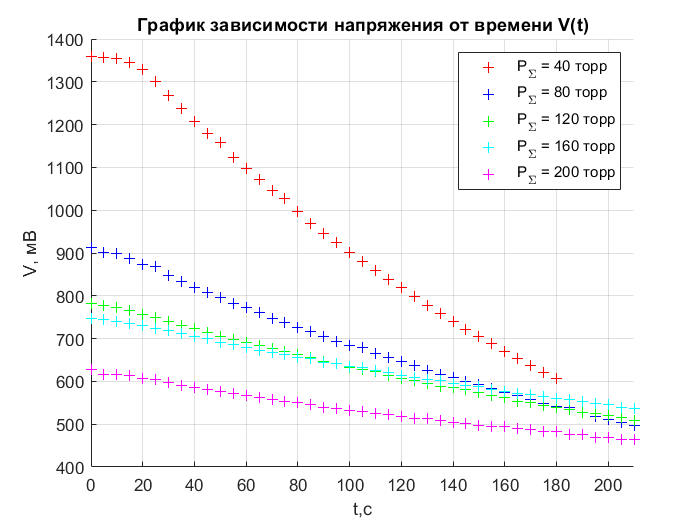
\includegraphics[width=0.5\linewidth]{graph_1.png}
\label{graph} 
\end{center}
\end{figure}
\paragraph{}
Видим, что при $P_{\Sigma} = 40$ торр и при $P_{\Sigma} = 80$ торр первые 3 значения не соответствуют общей тенденции графика $\Rightarrow$ при построении зависимости от $lnV(t)$ мы не будем включать эти точки в график

\item Для каждого из давлений построим графики, откладывая по
оси абсцисс время, а по оси ординат - логарифм от показаний гальванометра.

График будем строить, воспользовавшись методом наименьших квадратов $$ y = a + bx $$:
\begin{equation}
b = \frac{\langle xy \rangle - \langle x \rangle \langle y \rangle}{\langle x^2 \rangle - \langle x \rangle^2} \;\;
a = \langle y \rangle - b* \langle x \rangle
\label{mnk}
\end{equation}
Погрешность в этом случае можно найти по формуле: 
\begin{equation}
\sigma_b \approx \frac{1}{\sqrt{N}}\sqrt{\frac{\langle y^2 \rangle - \langle y \rangle ^ 2}{\langle x^2 \rangle - \langle x \rangle ^ 2} - b^2} ;\;\;\ \sigma_a \approx \sigma_b\sqrt{\lambda x^2 \rangle - \lambda x \rangle ^2} 
\end{equation}
\paragraph{График зависимости $lnV(t)$ $P_{\Sigma} = 40$ торр:}

Построим график зависимости $lnV(t)$ Здесь $x \Rightarrow t, y \Rightarrow \log V$. Для этого сперва определим константы, необходимые для подсчета коэффициента $b_1$ при данном значении давления:\\
$\langle t \rangle = 82,5$\\ 
$\langle \log V \rangle = 6,8154$\\
$\langle t^2 \rangle = 921,25$\\
$\langle \log V^2 \rangle = 46,5079$\\
$\langle t*\log V \rangle = 550,4822$\\
Всего бралось $ N = 34$ точек для аппроксимации. \\
Найдем константу:
\begin{equation*}
b_1 = \dfrac{550,4822 - 82,5*6,8154}{921,25 - 82,5^2} =  -0,0049 
\end{equation*}
\begin{equation*}
\sigma_{b_1} = \frac{1}{\sqrt{34}}\sqrt{\frac{46,5079 - 6,8154^2}{921,25 - 82,5^2} - 0,0049^2} = 0,1 * 10^{-3}
\end{equation*}
\begin{figure}[h]
\begin{center}
\begin{minipage}[h]{0.45\linewidth}
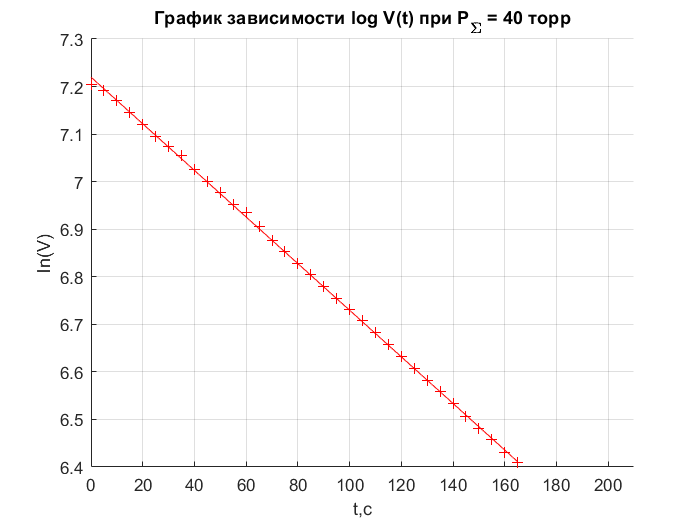
\includegraphics[width=1\linewidth]{gr_40_t.png}
\end{minipage}
\hfill
\begin{minipage}[h]{0.45\linewidth}
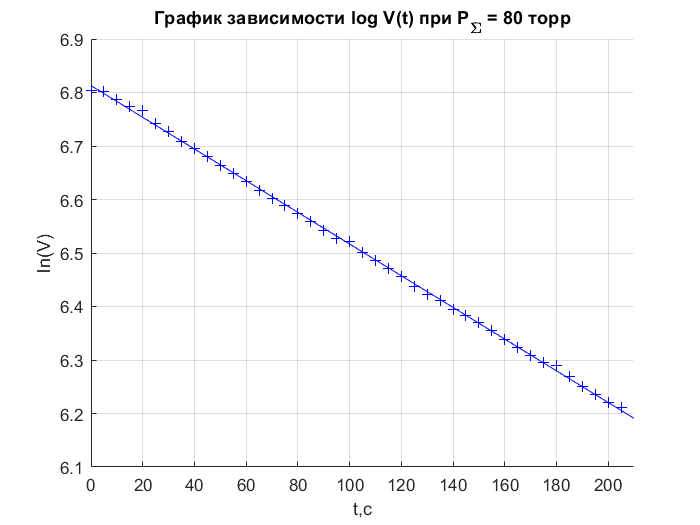
\includegraphics[width=1\linewidth]{gr_80_t.png}
\end{minipage}
\end{center}
\end{figure}
\paragraph{График зависимости $lnV(t)$ $P_{\Sigma} = 80$ торр:}

Определим константы, необходимые для подсчета коэффициента $b_2$ при данном значении давления:\\
$\langle t \rangle = 102,5$\\ 
$\langle \log V \rangle = 6,5093$\\
$\langle t^2 \rangle = 14179$\\
$\langle \log V^2 \rangle = 42,4037$\\
$\langle t*\log V \rangle = 656,3320$\\
Всего бралось $ N = 42$ точек для аппроксимации. \\
Найдем константу:
\begin{equation*}
b_2 = \dfrac{656,3320 - 102,5*6,5093}{14179 - 102,5^2} = -0,00296
\end{equation*}
\begin{equation*}
\sigma_{b_2} = \frac{1}{\sqrt{42}}\sqrt{\frac{42,4037 - 6,5093^2}{14179 - 102,5^2} - 0,00296^2} = 0,1 * 10^{-3}
\end{equation*}
\end{enumerate}

\paragraph{График зависимости $lnV(t)$ $P_{\Sigma} = 120$ торр:}

Определим константы, необходимые для подсчета коэффициента $b_3$ при данном значении давления:\\
$\langle t \rangle = 105$\\ 
$\langle \log V \rangle = 6,4460$\\
$\langle t^2 \rangle = 14875$\\
$\langle \log V^2 \rangle = 41,5676$\\
$\langle t*\log V \rangle = 668,7896$\\
Всего бралось $ N = 43$ точек для аппроксимации. \\
Найдем константу:
\begin{equation*}
b_3= \dfrac{668,7896 - 105*6,4460}{14875 - 105^2} = -0,00209
\end{equation*}
\begin{equation*}
\sigma_{b_3} = \frac{1}{\sqrt{43}}\sqrt{\frac{41,5676 - 6,4460^2}{14875 - 105^2} - 0,00209^2} = 0,1 * 10^{-3}
\end{equation*}
\begin{figure}[h]
\begin{center}
\begin{minipage}[h]{0.45\linewidth}
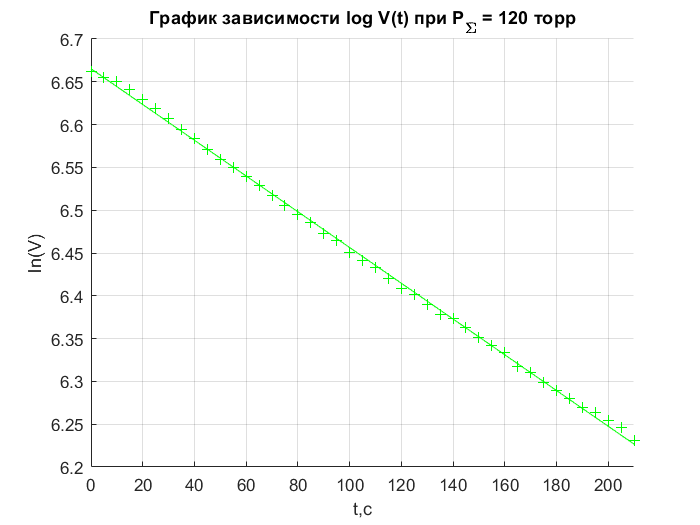
\includegraphics[width=1\linewidth]{gr_120_t.png}
\end{minipage}
\hfill
\begin{minipage}[h]{0.45\linewidth}
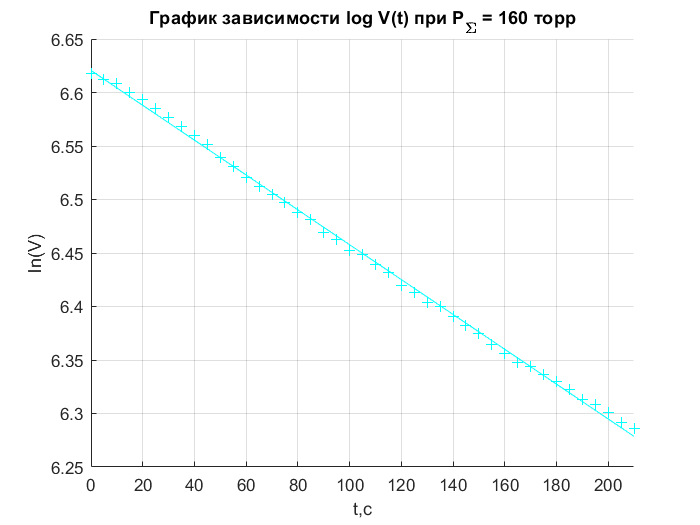
\includegraphics[width=1\linewidth]{gr_160_t.png}
\end{minipage}
\end{center}
\end{figure}
\paragraph{График зависимости $lnV(t)$ $P_{\Sigma} = 160$ торр:}

Определим константы, необходимые для подсчета коэффициента $b_4$ при данном значении давления:\\
$\langle t \rangle = 105$\\ 
$\langle \log V \rangle = 6,4496$\\
$\langle t^2 \rangle = 14875$\\
$\langle \log V^2 \rangle = 41,6076$\\
$\langle t*\log V \rangle = 670,9393$\\
Всего бралось $ N = 43$ точек для аппроксимации. \\
Найдем константу:
\begin{equation*}
b_4 =\dfrac{670,9393 - 105*6,4496}{14875 - 105^2} = -0,00163
\end{equation*}
\begin{equation*}
\sigma_{b_4} = \frac{1}{\sqrt{43}}\sqrt{\frac{41,6076 - 6,4492^2}{14875 - 105^2} - 0,00163^2} = 0,2 * 10^{-3}
\end{equation*}
\paragraph{График зависимости $lnV(t)$ $P_{\Sigma} = 200$ торр:}

Определим константы, необходимые для подсчета коэффициента $b_5$ при данном значении давления:\\
$\langle t \rangle = 105$\\ 
$\langle \log V \rangle = 6,2788$\\
$\langle t^2 \rangle = 14875$\\
$\langle \log V^2 \rangle = 39,4309$\\
$\langle t*\log V \rangle = 653,7311$\\
Всего бралось $ N = 43$ точек для аппроксимации. \\
Найдем константу:
\begin{equation*}
b_5 =\dfrac{653,7311 - 105*6,2788}{14875 - 105^2}= -0,0014
\end{equation*}
\begin{equation*}
\sigma_{b_5} = \frac{1}{\sqrt{43}}\sqrt{\frac{39,4309 - 6,2788^2}{14875 - 105^2} - 0,0014^2} = 0,2 * 10^{-3}
\end{equation*}
\begin{figure}[h]
\begin{center}
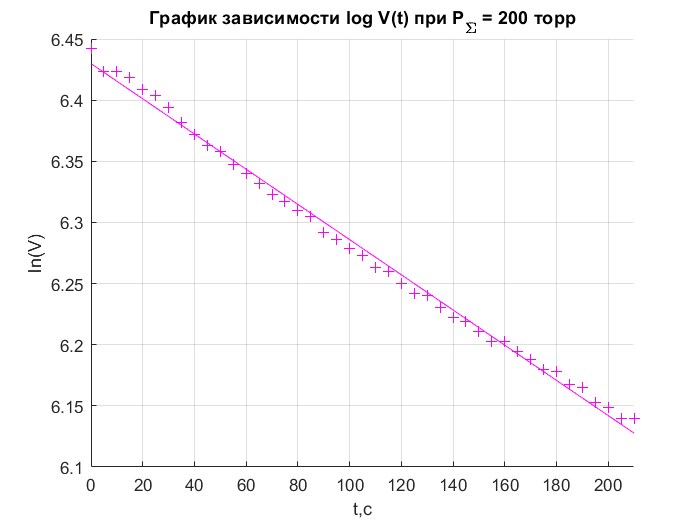
\includegraphics[width=0.5\linewidth]{gr_200_t.png}
\label{graph_200} 
\end{center}
\end{figure}

Построим сводный график:
\begin{figure}[h]
\begin{center}
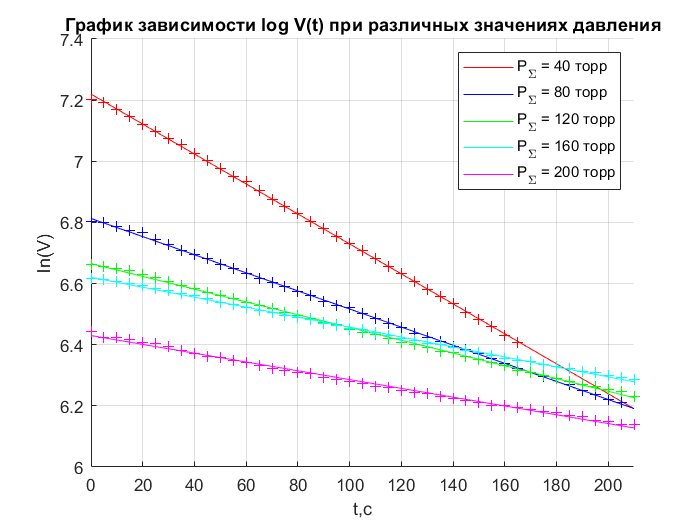
\includegraphics[width=0.5\linewidth]{graph_2.png}
\label{graph} 
\end{center}
\end{figure}

\paragraph{}
По угловым коэффициентам экспериментальных прямых и известным параметрам установки рассчитаем коэффициенты взаимной диффузии и их погрешности при выбранных давлениях по формулам:
\begin{equation} 
D =  -\frac{1}{2} Vb \frac{L}{S}
\end{equation}
\begin{equation}
\sigma_D = D \sqrt{\big(\frac{\sigma_b}{b}\big)^2 + \big(\frac{\sigma_V }{V}\big)^2 + \big(\frac{\sigma_{L/S}}{L/S}\big)^2}
\end{equation}
где $b$ - коэффициенты наклонов прямых
\begin{equation*} 
D_1 =  \frac{1}{2} 775*0,0049 *5,3 = 10,0634, \;\;\;\;\; \sigma_{D_1} = 10,0634*\sqrt{1*10^{-8} + 1,665 * 10^{-4} * 3,56 * 10^{-4}} = 0,3
\end{equation*}
\begin{equation*} 
D_2 =  \frac{1}{2} 775*0,00296 *5,3 = 6,0791, \;\;\;\;\; \sigma_{D_2} = 6,0791*\sqrt{1*10^{-8} + 1,665 * 10^{-4} * 3,56 * 10^{-4}} = 0,2
\end{equation*}
\begin{equation*} 
D_3 =  \frac{1}{2} 775*0,00209 *5,3 = 4,2923, \;\;\;\;\; \sigma_{D_3} = 4,2923*\sqrt{1*10^{-8} + 1,665 * 10^{-4} * 3,56 * 10^{-4}} = 0,1
\end{equation*}
\begin{equation*} 
D_4 =  \frac{1}{2} 775*0,00163 *5,3 = 3,3476, \;\;\;\;\; \sigma_{D_4} = 3,3476*\sqrt{4*10^{-8} + 1,665 * 10^{-4} * 3,56 * 10^{-4}} = 0,08
\end{equation*}
\begin{equation*} 
D_5 =  \frac{1}{2} 775*0,0014 *5,3 = 2,8752 , \;\;\;\;\; \sigma_{D_5} = 2,8752*\sqrt{4*10^{-8} + 1,665 * 10^{-4} * 3,56 * 10^{-4}} = 0,07
\end{equation*}
\paragraph{} 
Результаты сведены в таблицу:


\begin{tabular}{|l|l|l|l|l|l|}
\hline 
P, торр & 40 & 80 & 120 & 160 & 200 \\ 
\hline 
D, $\frac{\text{см}^2}{c}$ & 10,0634 & 6,0791 & 4,2923 & 3,3476 & 2,8752 \\ 
\hline 
$\sigma_{D}$,  $\frac{\text{см}^2}{c}$ & 0,3 & 0,2 & 0,1 & 0,08 & 0,07 \\ 
\hline 
\end{tabular} 
\paragraph{} 
 По полученным данным для коэффициента D, построим график зависимости D(1/P), пользуясь МНК:
 \begin{equation*}
b = \frac{\langle D*1/P \rangle - \langle 1/P \rangle \langle D \rangle}{\langle (1/P)^2 \rangle - \langle (1/P) \rangle ^ 2}, \;\;
a = \langle D \rangle - b \langle (1/P) \rangle  \label{lsf}
\end{equation*}
$\langle 1/P \rangle = 1,142*10^{-2}$\\ 
$\langle D \rangle = 5,333$\\
$\langle (1/P)^2 \rangle = 1,829 * 10^{-4}$\\
$\langle D^2 \rangle = 35,29$\\
$\langle D*(1/P) \rangle = 7,983 * 10^{-2}$\\
$N=5$
\begin{equation*}
b = \frac{7,983 * 10^{-2} - 1,142*10^{-2}*5,333}{1,829 * 10^{-4} - (1,142*10^{-2})^2} = 358,48 \;\;\;\;\;\; a = 5,333 - 358,48*1,142*10^{-2} = 1,24
\end{equation*}
\begin{figure}[h]
\begin{center}
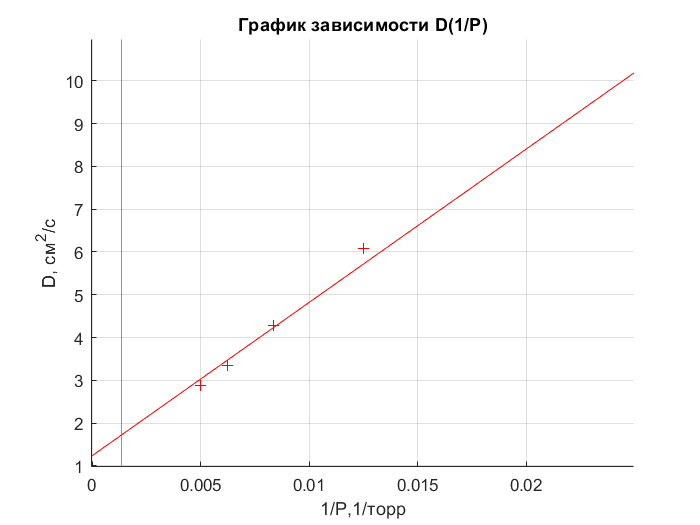
\includegraphics[width=0.5\linewidth]{graph_3.png}
\end{center}
\end{figure}
Найдем точку пересечения прямой x = 1/748 и y = 1,24 + 358,48x
Получим значение коэффициента взаимной диффузии:
$$D = 1,24 + 358,48 * (1/748) \approx 1,72 \frac{\text{см}^2}{c}$$
Оценим погрешность:
$$\sigma_{b} = \frac{1}{\sqrt{5}}\sqrt{\frac{35,29 - 5,333^2}{1,829*10^{-4} - 1,142*10^{-2}} - 358,48^2} = 11 $$
$$\sigma_{a} = \sigma_{b}\sqrt{1,829*10^{-4} - (1,142*10^{-2})^2} = 0,08$$
$$\sigma_{D} = D\sqrt{(\frac{\sigma_{b}}{b})^2 + (\frac{\sigma_{a}}{a})^2} = 1,72\sqrt{({\frac{11}{358,48}}^2) + ({\frac{0,08}{1,24}}^2)} \approx 0,1 $$
\section{Вывод:}
\begin{enumerate}
\itemsep0em
\item Подтвердили линейную зависимость $lnV(t)$
\item Установили линейную зависимость $D(1/P)$
\item Рассчитали коэффициенты взаимной диффузии при \\
$P_{\Sigma} = 40$ торр, равное $D_1 = 10,1 \pm 0,3 \frac{\text{см}^2}{c}$ \\
$P_{\Sigma} = 80$ торр, равное $D_2 = 6,1 \pm 0,2 \frac{\text{см}^2}{c}$ \\
$P_{\Sigma} = 120$ торр, равное $D_3 = 4,3 \pm 0,1 \frac{\text{см}^2}{c}$ \\
$P_{\Sigma} = 160$ торр, равное $D_4 = 3,35 \pm 0,08 \frac{\text{см}^2}{c}$ \\
$P_{\Sigma} = 200$ торр, равное $D_1 = 2,88 \pm 0,07 \frac{\text{см}^2}{c}$  
\item Получили численное значение коэффициента взаимной диффузии при давлении $P = 748$ торр, равное $D = 1,7 \pm 0,1 \dfrac{\text{см}^2}{c}$
\end{enumerate}

\end{document}
